%Preámbulo:  
\documentclass{article} %O cualquier otra clase.  
\usepackage[T1]{fontenc}  
\usepackage[utf8]{inputenc}  
\usepackage[english]{babel}  
\usepackage{amsmath,amssymb}
\usepackage[export]{adjustbox}
\usepackage[affil-it]{authblk}
\usepackage[center]{caption}
\usepackage{hyperref}
\hypersetup{
    colorlinks=true,
    linkcolor=black,      
    pdftitle={Nuclear Physics - Computer Lab 1},
    }
\usepackage{graphicx}
\graphicspath{ {C:/Users/luisf/OneDrive - UNIVERSIDAD ALICANTE/UA/Física/Cuarto/1º Cuatrimestre/Física nuclear y de partículas/Práctica 1/Images} }
\author{Luis Lucas García}
\title{Answers to the analysis questions proposed for practice 1}
\date{\today}
\affil{Facultad de ciencias - Universidad de Alicante - Física nuclear y de partículas - Grupo L3 - Grado en física}
%Documento
\begin{document}
\maketitle
\begin{abstract}
In this document we will answer the questions proposed in the script for exercise 1 of the nuclear physics computer lab. We will analyze the binding energy for uranium and discuss how its fission works and how viable it is.
\end{abstract}
\tableofcontents

\section{Binding energy of Uranium}

We will begin by coding a calculator for the binding energy using the semi-empirical mass formula, given by:

\begin{equation}
B(Z, A) = a_v A -a_s A^{\frac{2}{3}} - a_c \frac{Z^2}{A^{\frac{1}{3}}} - a_a \frac{(A-2Z)^2}{A} + a_p \frac{(-1)^N + (-1)^Z}{2 \sqrt{A}}
\end{equation}

Where the constants are determined empirically and their values are given in the script of the exercise.

\subsection{Binding energy for U-238 and U-235}

Using the expression from before, we can calculate the binding energy per nucleon for these two isotopes. We use that for uranium, $Z = 92$ and then, we calculate:

$$
\begin{array}{cc}
\frac{B(92, 235)}{235} = 7.575 MeV & \frac{B(92, 238)}{238} = 7.558 MeV
\end{array}
$$

\subsection{Stability analysis}

Given the results from the last section, it can be seen that U-235 has a higher binding energy, which means that it's a more stable isotope of Uranium than U-238. This can be seen in the figure (\ref{fig:UIsot}).

\begin{figure}[h!]
\begin{center}
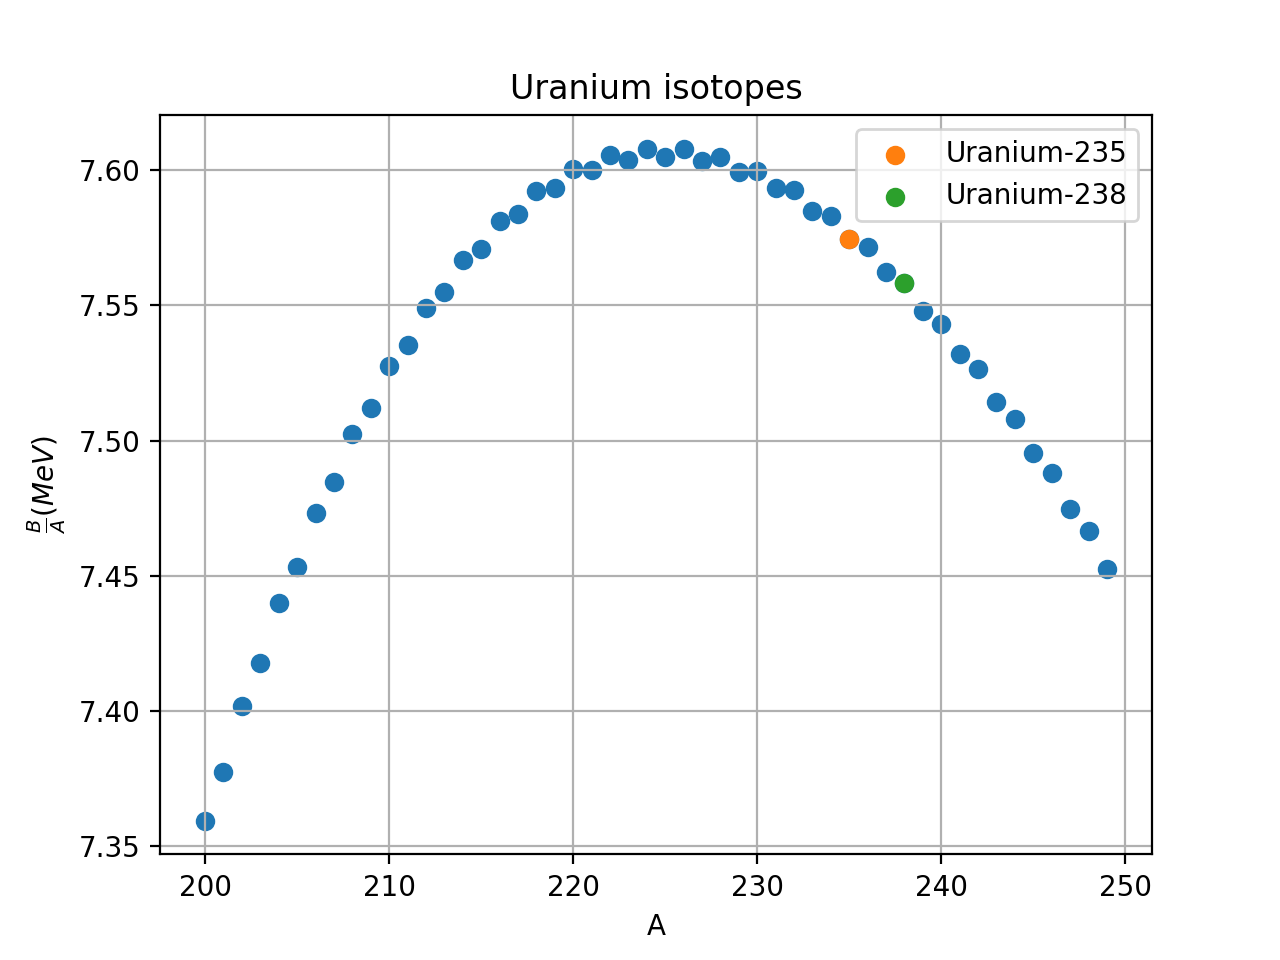
\includegraphics[max width=\linewidth]{Uranium Isotopes}
\caption{Binding energy per nucleon for different isotopes of uranium.}
\label{fig:UIsot}
\end{center}
\end{figure}

\section{Fission of Uranium}

The fission of uranium is given by the next expression:

\begin{equation}
^{238}_{92}U \rightarrow ^{92}_{36}Kr + ^{141}_{56}Ba
\end{equation}

In which the energy released in the reaction can be calculated using the difference of the binding energy between the products and the reactants.

\subsection{Calculation of binding energies}

We will begin by calculating the binding energies for each of the components of this reaction. In this case we have:

$$
\begin{array}{cc}
B(92, 238) = 1798.898 MeV & B(36, 92) = 775.977 MeV
\end{array}
$$
$$
B(56, 141) = 1163.474 MeV
$$

\subsection{Fission viability}

It can be directly seen that the summed energy of both of the products is higher than the binding energy of the Uranium-238, this means that this fission is a viable process.

We have to give the uranium its binding energy to break it apart, then, when the product nuclei are formed, their binding energy is released. Since they sum up to a higher binding energy, the products give enough energy to break the uranium atom and even release some energy as part of their formation which makes the fission viable.

\subsection{Energy released}

Using the difference between binding energies, we can calculate the energy released in the fission, it will be:

$$
E_r = B(36, 92) + B(56, 141) - B(92, 238) = 140.552 MeV
$$

Heavy nuclei tend to undergo fission because of their high mass. This high mass gives a lower binding energy, which means that when it breaks up its products will be more stable, since they will have a higher binding energy, this is why they undergo fission more often. This can be seen in figure (\ref{fig:BindingE}).

\begin{figure}[h!]
\begin{center}
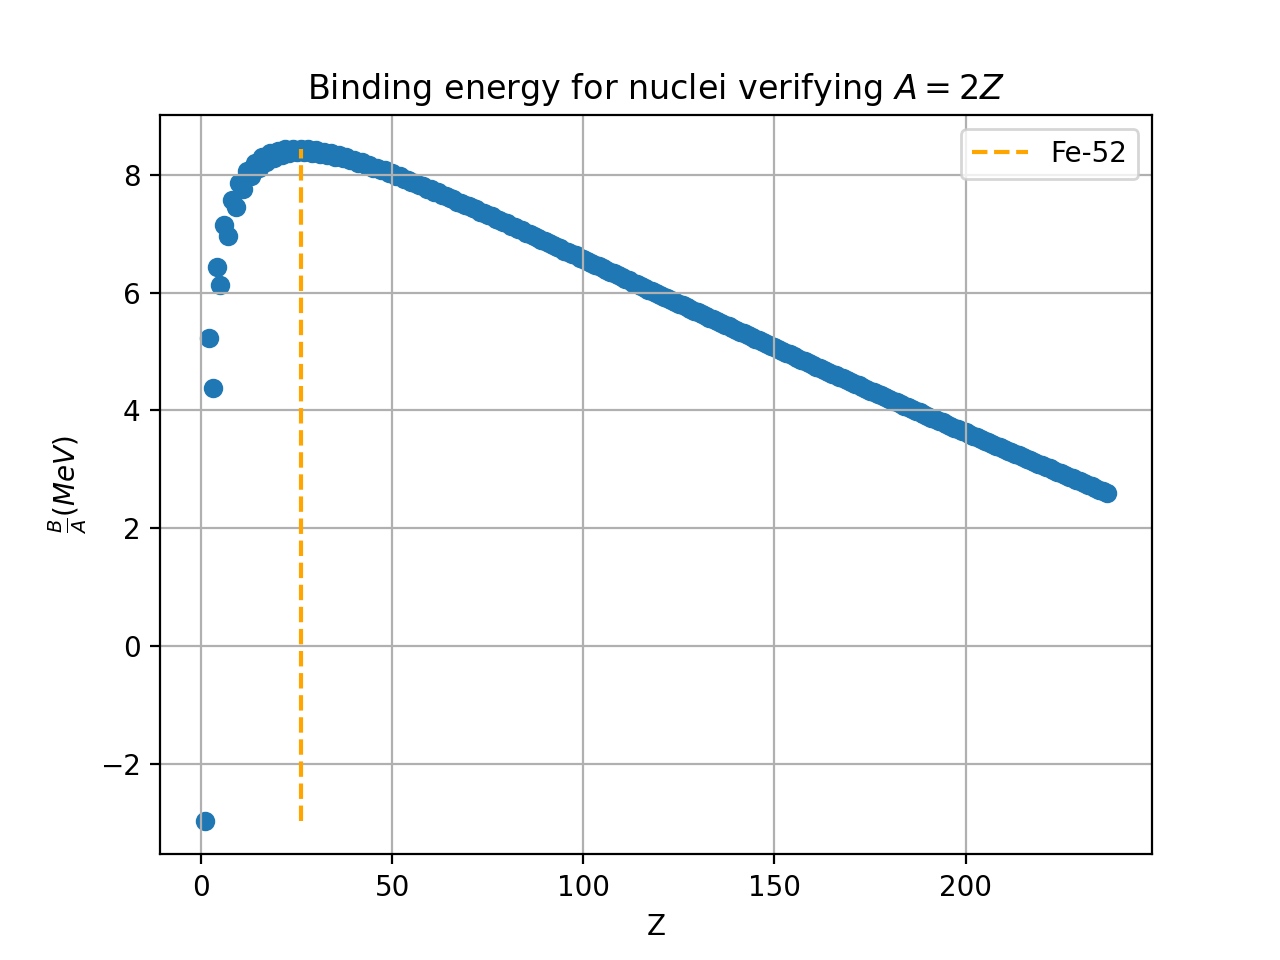
\includegraphics[max width=\linewidth]{Bounding energy}
\caption{Bounding energy per nucleon of nuclei verifying $A = 2Z$}
\label{fig:BindingE}
\end{center}
\end{figure}

\subsection{Comparisson of energies}

If we plot the total binding energies in a bar graph we can compare them. This can be seen in figure (\ref{fig:ECompar}).

\begin{figure}[h!]
\begin{center}
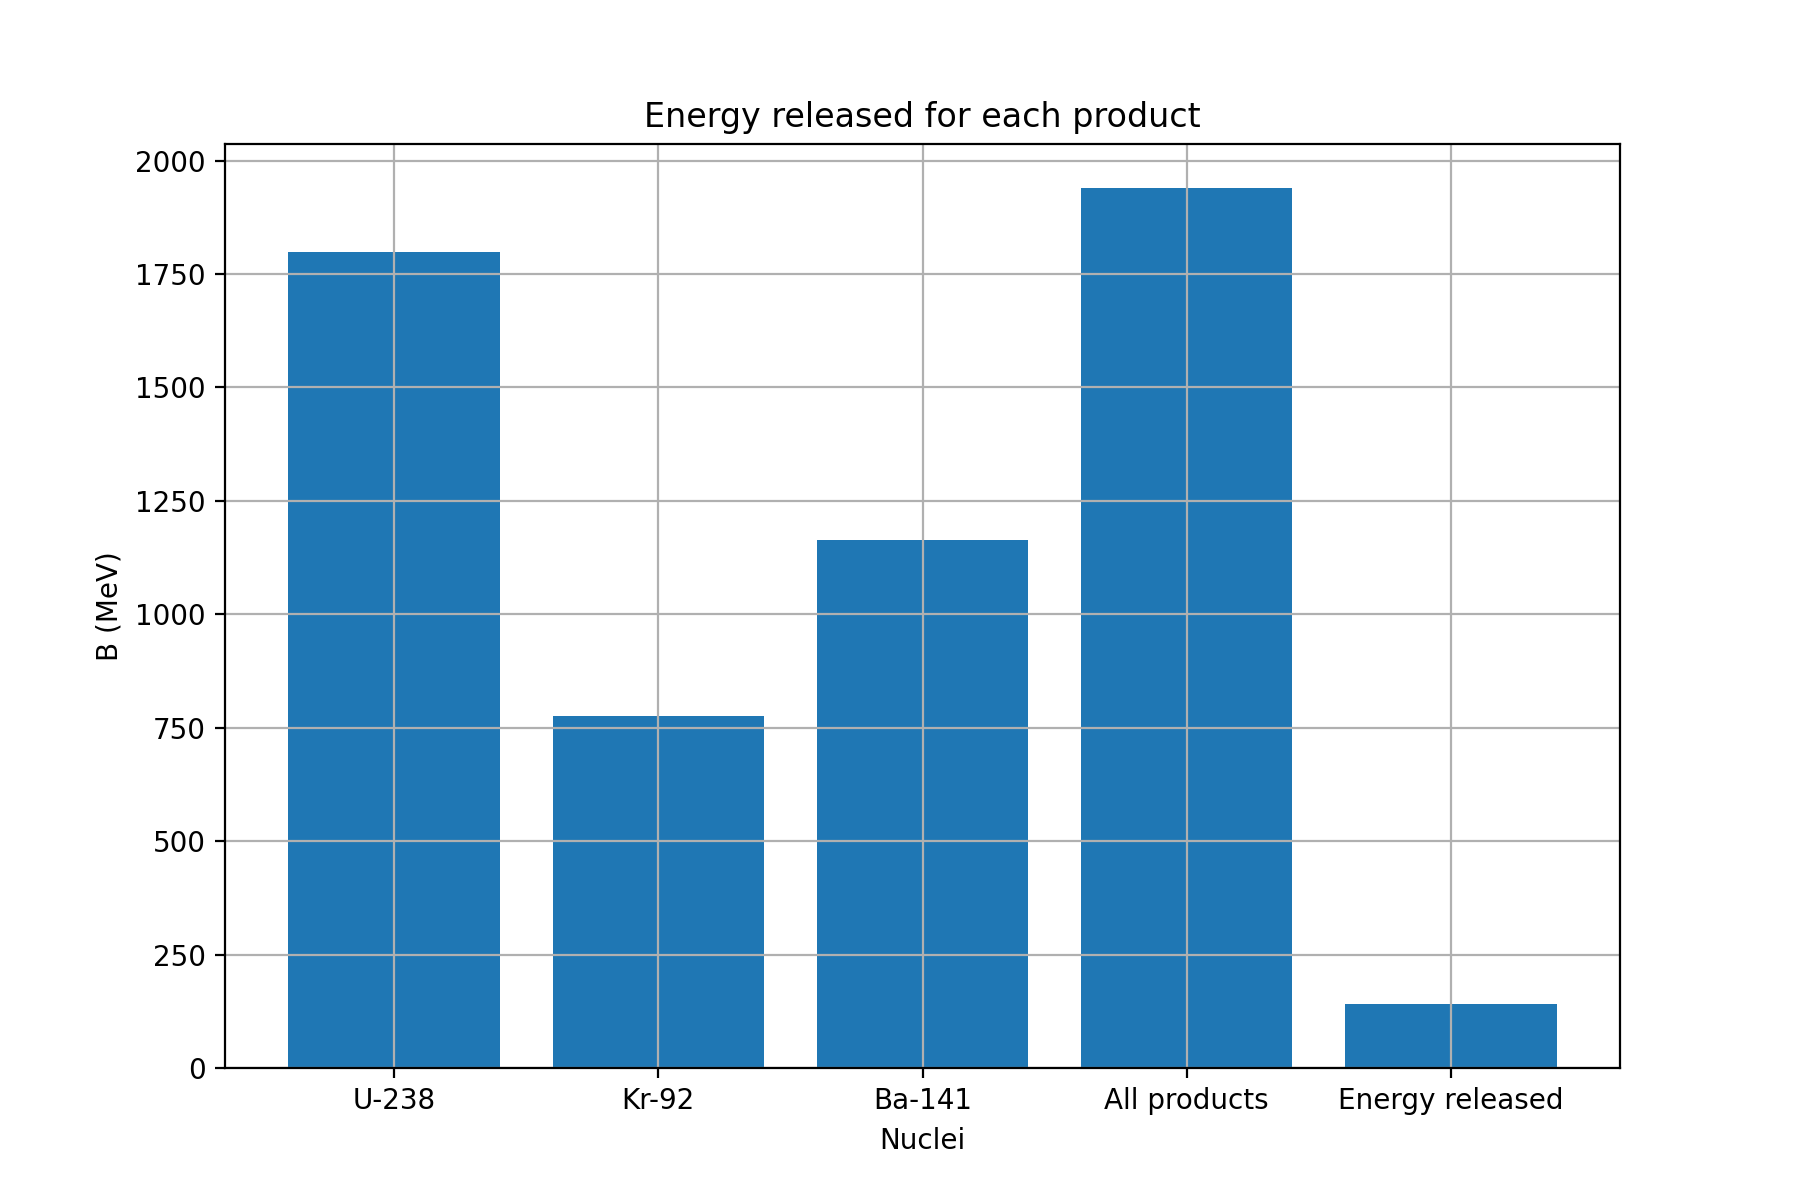
\includegraphics[max width=\linewidth]{Fission energy}
\caption{Bar plot of the fission energy of products and reactants, as well as released total energy.}
\label{fig:ECompar}
\end{center}
\end{figure}

We can see that, as we discused earlier, the energy of the products is higher than that of Uranium-238 which makes the reaction possible. We can also see that the energy produced is in the order of 10\% of the energy of the reactant.

\subsection{Comparison of energies}

The energy released is 7.81\% of the binding energy of the Uranium-238. However, this is not the used isotope in nuclear reactors, it's Uranium-235. This isotope is easier to concentrate to the point needed in nuclear reactors, however, the rate of energy released is of around 6.1\% of its binding energy if we study it's fission:

$$
n + ^{235}U \rightarrow ^{236}U \rightarrow 3n + ^{144}Ba + ^{89}Kr
$$

So, Uranium-238 would seem a better fuel for reactors, but since it doesn't generate neutrons is not interesting since it cannot produce a chain reaction that would trigger the consecutive fission of multiple nuclei.

Since U-238 is a less stable isotope it gives more energy when it's fissioned but it's harder to produce and doesn't gives way to a chain reaction, this is why Uranium-235 is mostly used in most applications.

\section{Conclussions}

In this document we have studied the viability of uranium-238 fissions. We have determined that it's a more unstable nuclei than the more used uranium-235, but, unlike the former one, it doesn't produce neutrons and it can't be used as fuel for a chain reactions, such as in nuclear reactors.

This exercise is interesting in a practical and educational way, to visualize the semi-empirical equation of masses and discuss some nuclear reactions. It is useful as an exercise in the nuclear physics class for the first part of the course as a tool to understand better the concepts studied in class.
\end{document}